\let\negmedspace\undefined
\let\negthickspace\undefined
\documentclass[journal,12pt,onecolumn]{IEEEtran}
\usepackage{cite}
\usepackage{amsmath,amssymb,amsfonts,amsthm}
\usepackage{algorithmic}
\usepackage{graphicx}
\graphicspath{{./figs/}}
\usepackage{textcomp}
\usepackage{xcolor}
\usepackage{txfonts}
\usepackage{listings}
\usepackage{enumitem}
\usepackage{mathtools}
\usepackage{gensymb}
\usepackage{comment}
\usepackage{caption}
\usepackage[breaklinks=true]{hyperref}
\usepackage{tkz-euclide} 
\usepackage{listings}
\usepackage{gvv}                                        
%\def\inputGnumericTable{}                                 
%\usepackage[latin1]{inputenc}     
\usepackage{xparse}
\usepackage{color}                                            
\usepackage{array}                                            
\usepackage{longtable}                                       
\usepackage{calc}                                             
\usepackage{multirow}
\usepackage{multicol}
\usepackage{hhline}                                           
\usepackage{ifthen}                                           
\usepackage{lscape}
\usepackage{tabularx}
\usepackage{array}
\usepackage{float}
\newtheorem{theorem}{Theorem}[section]
\newtheorem{problem}{Problem}
\newtheorem{proposition}{Proposition}[section]
\newtheorem{lemma}{Lemma}[section]
\newtheorem{corollary}[theorem]{Corollary}
\newtheorem{example}{Example}[section]
\newtheorem{definition}[problem]{Definition}
\newcommand{\BEQA}{\begin{eqnarray}}
\newcommand{\EEQA}{\end{eqnarray}}
\newcommand{\define}{\stackrel{\triangle}{=}}
\theoremstyle{remark}
\newtheorem{rem}{Remark}

\setlength{\tabcolsep}{15pt}
\renewcommand{\arraystretch}{1.75}

\begin{document}

\title{GATE 2023-CE}
\author{Pratyush Panda(AI25BTECH11024)}
\maketitle

\renewcommand{\thefigure}{\theenumi}
\renewcommand{\thetable}{\theenumi}

\section*{Q. 1-Q. 20 carry one mark each.}

\begin{enumerate}
\item  The minimum and the maximum eigen values of the matrix $\myvec{1 & 1 & 3\\1 & 5 & 1\\3 & 1 & 1}$ are $-2$ and $6$ respectively. What are the other eigen values?

\hfill{\brak{\text{GATE CE 2007}}}
\begin{enumerate}
\item 3
\item 5
\item 1
\item -1
\end{enumerate}

\item The degree of the differential equation $\frac{d^2x}{dt^2}+2x^3=0$ is

\hfill{\brak{\text{GATE CE 2007}}}
\begin{enumerate}
\item 0
\item 1
\item 2
\item 3
\end{enumerate}

\item The solution of the differential equation $\frac{dy}{dx}=x^2y$ with the condition that $y=1$ at $x=0$ is

\hfill{\brak{\text{GATE CE 2007}}}
\begin{enumerate}
\item $y=e^{\frac{1}{2x}}$
\item $ln(y)=\dfrac{x^3}{3}+4$
\item $ln(y)=\dfrac{x^2}{2}$
\item $y=e^{\frac{x^3}{3}}$
\end{enumerate}

\item An axially loaded bar is subjected to a normal stress of $173MPa$. The shear stress in the bar is

\hfill{\brak{\text{GATE CE 2007}}}
\begin{enumerate}
\item $75MPa$
\item $86.5MPa$
\item $100MPa$
\item $122.3MPa$
\end{enumerate}

\item A steel column, pinned at both ends, has a buckling load of $200kN$. If the column is restricted against lateral movement at its mid-height, its buckling load will be

\hfill{\brak{\text{GATE CE 2007}}}
\begin{enumerate}
\item $200kN$
\item $283kN$
\item $400kN$
\item $800kN$
\end{enumerate}

\item The stiffness coefficient $k_{ij}$ indicates

\hfill{\brak{\text{GATE CE 2007}}}
\begin{enumerate}
\item force at i due to a unit deformation at j
\item deformation at j due to a unit force at i
\item deformation at i due to a unit force at j
\item force at j due to a unit deformation at i
\end{enumerate}

\item For an isotropic material, the relationship between the Young's modulus $\brak{\text{E}}$, shear modulus $\brak{\text{G}}$ and poisson's ratio $\brak{\mu}$ is given by

\hfill{\brak{\text{GATE CE 2007}}}
\begin{enumerate}
\item $G=\dfrac{E}{2(1+\mu)}$
\item $E=\dfrac{G}{2(1+\mu)}$
\item $G=\dfrac{E}{(1+2\mu)}$
\item $G=\dfrac{E}{2(1-\mu)}$
\end{enumerate}

\item  A clay soil sample is tested in a triaxial apparatus in consolidated-drained conditions at a cell pressure of $100 kN/m^2$. What will be the pore water pressure at a deviator stress of $40 kN/m^2$?

\hfill{\brak{\text{GATE CE 2007}}}
\begin{enumerate}
\item $0kN/m^2$
\item $20kN/m^2$
\item $40kN/m^2$
\item $60kN/m^2$
\end{enumerate}

\item The number of blows observed in a Standard Penetration Test $\brak{\text{SPT}}$ for different penetration depths are given as follows:

\hfill{\brak{\text{GATE CE 2007}}}
\begin{table}[H]
\centering
\begin{tabular}{c|c}
Penetration of sample & Number of blows\\
\hline
$0-150mm$ & 6\\
\hline
$150-300mm$ & 8\\
\hline
$300-450mm$ & 10\\
\end{tabular}
\caption*{}
\label{tab:Q.9}
\end{table}
The observed N value is

\begin{enumerate}
\item 8
\item 14
\item 18
\item 24
\end{enumerate}

\item The vertical stress at some depth below the corner of a $2m\times3m$ rectangular footing due to a certain load intensity is $100 kN/m^2$. What will be the vertical stress in $kN/m^2$ below the centre of a $4m\times6m$ rectangular footing at the same depth and same load intensity?

\hfill{\brak{\text{GATE CE 2007}}}
\begin{enumerate}
\item 25
\item 100
\item 200
\item 400
\end{enumerate}

\item There is a free overfall at the end of a long open channel. For a given flow rate, the critical depth is less than the normal depth. What gradually varied flow profile will occur in the channel for this flow rate?

\hfill{\brak{\text{GATE CE 2007}}}
\begin{enumerate}
\item $M_1$
\item $M_2$
\item $M_3$
\item $S_1$
\end{enumerate}

\item The consumptive use of water for a crop during a particular stage of growth is $2.0 mm/day$. The maximum depth of available water in the root zone is $60 mm$. Irrigation is required when the amount of available water is 50\% of the maximum available water in the root zone. Frequency of irrigation should be

\hfill{\brak{\text{GATE CE 2007}}}
\begin{enumerate}
\item 10 days
\item 15 days
\item 20 days
\item 25 days
\end{enumerate}

\item As per the Lacey's method for design of alluvial channels, identify the TRUE statement from the following:

\hfill{\brak{\text{GATE CE 2007}}}
\begin{enumerate}
\item Wetted perimeter increases with an increase in design discharge.
\item Hydraulic radius increases with an increase in silt factor.
\item Wetted perimeter decreases with an increase in design discharge.
\item Wetted perimeter increases with an increase in silt factor.
\end{enumerate}

\item At two points 1 and 2 in a pipeline the velocities are V and 2V, respectively. Both the points are at the same elevation. The fluid density is p. The flow can be assumed to be incompressible, inviscid, steady and irrotational. The difference in pressures $P_1$ and $P_2$ at points 1 and 2 is

\hfill{\brak{\text{GATE CE 2007}}}
\begin{enumerate}
\item $0.5\rho V^2$
\item $1.5\rho V^2$
\item $2\rho V^2$
\item $3\rho V^2$
\end{enumerate}

\item  The presence of hardness in excess of permissible limit causes

\hfill{\brak{\text{GATE CE 2007}}}
\begin{enumerate}
\item cardio vascular problems.
\item skin discolouration.
\item calcium deficiency.
\item increased laundry expenses.
\end{enumerate}

\item The dispersion of pollutants in atmosphere is maximum when

\hfill{\brak{\text{GATE CE 2007}}}
\begin{enumerate}
\item environmental lapse rate is greater than adiabatic lapse rate.
\item environmental lapse rate is less than adiabatic lapse rate. 
\item environmental lapse rate is equal to adiabatic lapse rate.
\item maximum mixing depth is equal to zero.
\end{enumerate}

\item The alkalinity and the hardness of a water sample are $250 mg/L$ and $350 mg/L$ as $CaCO_3$, respectively. The water has

\hfill{\brak{\text{GATE CE 2007}}}
\begin{enumerate}
\item $350 mg/L$ carbonate hardness and zero non-carbonate hardness.
\item $250 mg/L$ carbonate hardness and zero non-carbonate hardness.
\item $250 mg/L$ carbonate hardness and 350 mg/L non-carbonate hardness.
\item 250 mg/I. carbonate hardness and 100 mg/L non-carbonate hardness.
\end{enumerate}

\item The consistency and flow resistance of bitumen can be determined from the following:

\hfill{\brak{\text{GATE CE 2007}}}
\begin{enumerate}
\item Ductility test
\item Penetration test
\item Softening point test
\item Viscosity test
\end{enumerate}

\item If a two-lane national highway and a two-lane state highway intersect at right angles, the number of potential conflict points at the intersection, assuming that both the roads are two-way is

\hfill{\brak{\text{GATE CE 2007}}}
\begin{enumerate}
\item 11
\item 17
\item 24
\item 32
\end{enumerate}

\item In signal design as per Indian Roads Congress specifications, if the sum of the ratios of normal flows to saturation flow of two directional traffic flow is $0.50$ and the total lost time per cycle is $10 \, seconds$, the optimum cycle length in seconds is

\hfill{\brak{\text{GATE CE 2007}}}
\begin{enumerate}
\item 100
\item 80
\item 60
\item 40
\end{enumerate}

\section*{Q. 21 to Q. 75 carry two marks each.}

\item For what values of $\alpha$ and $\beta$ the following simultaneous equations have an infinite number of solutions?
$x+y+z=5; \hspace{0.5cm} x+3y+3z=9; \hspace{0.5cm} x+2y+\alpha z=\beta$

\hfill{\brak{\text{GATE CE 2007}}}
\begin{enumerate}
\item 2,7
\item 3,8
\item 8,3
\item 7,2
\end{enumerate}

\item A velocity vector is given as $\vec{V} = 5x\hat{i} + 2y^2\hat{j} + 3yz^2\hat{k}$. The divergence of this velocity vector at $\brak{1,1,1}$ is

\hfill{\brak{\text{GATE CE 2007}}}
\begin{enumerate}
\item 9
\item 10
\item 14
\item 15
\end{enumerate}

\item A body originally at $60^\circ$C cools down to $40^\circ$C in 15 minutes when kept in air at a temperature of $25^\circ$C. What will be the temperature of the body at the end of 30 minutes?

\hfill{\brak{\text{GATE CE 2007}}}

\begin{enumerate}
\item 35.2$^\circ$C
\item 31.5$^\circ$C
\item 28.7$^\circ$C
\item 15$^\circ$C
\end{enumerate}

\item The following equation needs to be numerically solved using the Newton-Raphson method. $x^3 + 4x - 9 = 0$
The iterative equation for this purpose is $\brak{\text{k indicates the iteration level}}$
\hfill{\brak{\text{GATE CE 2007}}}
\begin{enumerate}
\item $x_{k+1} = \dfrac{2x_k^3 + 9}{3x_k^2 + 4}$
\item $x_{k+1} = \dfrac{2x_k^3 + 9}{3x_k^2 + 9}$
\item $x_{k+1} = x_k - \frac{x_k^3 + 4x_k - 9}{3x_k^2 + 4}$
\item $x_{k+1} = \dfrac{4x_k^2 + 3}{9x_k^2 + 2}$
\end{enumerate}

\item Evaluate $\int_0^\pi \frac{\sin t}{t} dt$
\hfill{\brak{\text{GATE CE 2007}}}
\begin{enumerate}
\item $\pi$
\item $\pi/2$
\item $\pi/4$
\item $\pi/8$
\end{enumerate}

\item Potential function $\phi$ is given as $\phi = x^2 - y^2$. What will be the stream function $(\psi)$ with the condition $\psi = 0$ at $x = y = 0$?
\hfill{\brak{\text{GATE CE 2007}}}
\begin{enumerate}
\item $2xy$
\item $x^2 + y^2$
\item $x^2 - y^2$
\item $2x^2y^2$
\end{enumerate}

\item The inverse of the $2 \times 2$ matrix $\myvec{1 & 2 \\ 5 & 7}$ is,

\hfill{\brak{\text{GATE CE 2007}}}
\begin{enumerate}
\item $\dfrac{1}{3}\myvec{-7 & 2 \\ 5 & -1}$
\item $\dfrac{1}{3}\myvec{7 & 2 \\ 5 & 1}$
\item $\dfrac{1}{3}\myvec{7 & -2 \\ -5 & 1}$
\item $\dfrac{1}{3}\myvec{-7 & -2 \\ -5 & -1}$
\end{enumerate}

\item Given that one root of the equation $x^3 - 10x^2 + 31x - 30 = 0$ is 5, the other two roots are

\hfill{\brak{\text{GATE CE 2007}}}
\begin{enumerate}
\item 2 and 3
\item 2 and 4
\item 3 and 4
\item -2 and -3
\end{enumerate}

\item If the standard deviation of the spot speed of vehicles in a highway is $8.8 kmph$ and the mean speed of the vehicles is $33 kmph$, the coefficient of variation in speed is

\hfill{\brak{\text{GATE CE 2007}}}
\begin{enumerate}
\item 0.1517
\item 0.1867
\item 0.2666
\item 0.3646
\end{enumerate}

\item A metal bar of length 100 mm is inserted between two rigid supports and its temperature is increased by $10^\circ$C. If the coefficient of thermal expansion is $12 \times 10^{-6}$ per $^\circ$C and the Young’s modulus is $2 \times 10^5 MPa$, the stress in the bar is

\hfill{\brak{\text{GATE CE 2007}}}
\begin{enumerate}
\item zero
\item $12 MPa$
\item $24 MPa$
\item $2400 MPa$
\end{enumerate}

\item A rigid bar is suspended by three rods made of the same material as shown in the figure. The area and length of the central rod are $3A$ and $L$, respectively, while that of the two outer rods are $2A$ and $2L$, respectively. If a downward force of $50 kN$ is applied to the rigid bar, the forces in the central and each of the outer rods will be

\hfill{\brak{\text{GATE CE 2007}}}
\begin{figure}[H]
\centering
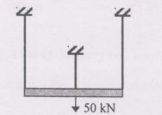
\includegraphics[width=0.3\columnwidth]{figs/q31.png}
\caption*{}
\label{fig:Q.31}
\end{figure}
\begin{enumerate}
\item $16.67 kN$ each
\item $30 kN$ and $15 kN$
\item $30 kN$ and $10 kN$
\item $21.4 kN$ and $14.3 kN$
\end{enumerate}

\item The maximum and minimum shear stresses in a hollow circular shaft of outer diameter $20 mm$ and thickness $2 mm$, subjected to a torque of $92.7 N.m$ will be

\hfill{\brak{\text{GATE CE 2007}}}

\begin{enumerate}
\item $59 MPa$ and $47.2 MPa$
\item $100 MPa$ and $80 MPa$
\item $118 MPa$ and $160 MPa$
\item $200 MPa$ and $160 MPa$
\end{enumerate}

\item The shear stress at the neutral axis in a beam of triangular section with a base of $40 mm$ and height $20 mm$, subjected to a shear force of $3 kN$ is

\hfill{\brak{\text{GATE CE 2007}}}

\begin{enumerate}
\item $3 MPa$
\item $6 MPa$
\item $10 MPa$
\item $20 MPa$
\end{enumerate}

\item $U_1$ and $U_2$ are the strain energies stored in a prismatic bar due to axial tensile forces $P_1$ and $P_2$, respectively. The strain energy $U$ stored in the same bar due to combined action of $P_1$ and $P_2$ will be

\hfill{\brak{\text{GATE CE 2007}}}

\begin{enumerate}
\item $U = U_1 + U_2$
\item $U = U_1 \, U_2$
\item $U < U_1 + U_2$
\item $U > U_1 + U_2$
\end{enumerate}

\item The right triangular truss is made of members having equal cross sectional area of $1550 mm^2$ and Young’s modulus of $2\times10^5 MPa$. The horizontal deflection of the joint Q is

\hfill{\brak{\text{GATE CE 2007}}}
\begin{figure}[H]
\centering
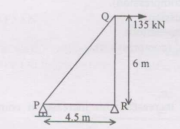
\includegraphics[width=0.3\columnwidth]{figs/q35.png}
\caption*{}
\label{fig:Q.35}
\end{figure}
\begin{enumerate}
\item $2.47 mm$
\item $10.25 mm$
\item $14.31 mm$
\item $15.68 mm$
\end{enumerate}

\item The influence line diagram $\brak{\text{ILD}}$ shown is for the member

\hfill{\brak{\text{GATE CE 2007}}}
\begin{figure}[H]
\centering
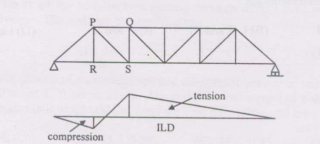
\includegraphics[width=0.4\columnwidth]{figs/q36.png}
\caption*{}
\label{fig:Q.36}
\end{figure}
\begin{enumerate}
\item PS
\item RS
\item PQ
\item QS
\end{enumerate}

\item Consider the following statements:

\begin{enumerate}
\item The compressive strength of concrete decreases with increase in water-cement ratio of the concrete mix.
\item Water is added to the concrete mix for hydration of cement and workability.
\item Creep and shrinkage of concrete are independent of the water-cement ratio in the concrete mix.
\end{enumerate}
The TRUE statements are

\hfill{\brak{\text{GATE CE 2007}}}
\begin{enumerate}
\item I and II
\item I, II and III
\item II and III
\item only II
\end{enumerate}

\item The percentage loss of prestress due to anchorage slip of 3 mm in a concrete beam of length 30 m which is post-tensioned by a tendon with an initial stress of 1200 N/mm$^2$ and modulus of elasticity equal to $2.1\times10^5$ N/mm$^2$ is

\hfill{\brak{\text{GATE CE 2007}}}
\begin{enumerate}
\item 0.0175
\item 0.175
\item 1.75
\item 17.5
\end{enumerate}

\item A concrete beam of rectangular cross-section of size 120 mm (width) and 200 mm (depth) is prestressed by a straight tendon to an effective force of 150 kN at an eccentricity of 20 mm (below the centroidal axis in the depth direction). The stresses at the top and bottom fibres of the section are

\hfill{\brak{\text{GATE CE 2007}}}
\begin{enumerate}
\item 2.5 N/mm$^2$ (compression), 10 N/mm$^2$ (compression).
\item 10 N/mm$^2$ (tension), 2.5 N/mm$^2$ (compression).
\item 3.75 N/mm$^2$ (tension), 3.75 N/mm$^2$ (compression).
\item 2.75 N/mm$^2$ (compression), 3.75 N/mm$^2$ (compression).
\end{enumerate}

\item Consider the following statements:

\begin{enumerate}
\item Modulus of elasticity of concrete increases with increase in compressive strength of concrete.
\item Brittleness of concrete increases with decrease in compressive strength of concrete.
\item Shear strength of concrete increases with increase in compressive strength of concrete.
\end{enumerate}

The TRUE statements are

\hfill{\brak{\text{GATE CE 2007}}}
\begin{enumerate}
\item II and III
\item I, II and III
\item I and II
\item I and III
\end{enumerate}

\item A steel flat of rectangular section of size $70 \times 6$ mm is connected to a gusset plate by three bolts each having a shear capacity of $15 kN$ in holes having diameter $11.5 mm$. If the allowable tensile stress in the flat is $150 MPa$, the maximum tension that can be applied to the flat is

\hfill{\brak{\text{GATE CE 2007}}}
\begin{figure}[H]
\centering
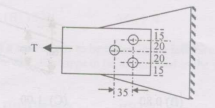
\includegraphics[width=0.3\columnwidth]{figs/q41.png}
\caption*{}
\label{fig:Q.41}
\end{figure}
\begin{enumerate}
\item 42.3 kN
\item 52.65 kN
\item 59.5 kN
\item 63.0 kN
\end{enumerate}

\item A bracket connection is made with four bolts of 10 mm diameter and supports a load of 10 kN at an eccentricity of 100 mm. The maximum force to be resisted by any bolt will be

\hfill{\brak{\text{GATE CE 2007}}}
\begin{figure}[H]
\centering
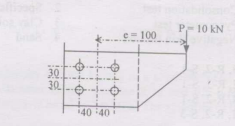
\includegraphics[width=0.3\columnwidth]{figs/q42.png}
\caption*{}
\label{fig:Q.42}
\end{figure}
\begin{enumerate}
\item 5 kN
\item 6.5 kN
\item 6.8 kN
\item 7.16 kN
\end{enumerate}

\item The plastic collapse load $W_p$ for the propped cantilever supporting two point loads as shown in figure in terms of plastic moment capacity, $M_p$, is given by

\hfill{\brak{\text{GATE CE 2007}}}
\begin{figure}[H]
\centering
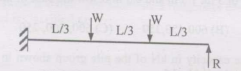
\includegraphics[width=0.3\columnwidth]{figs/q43.png}
\caption*{}
\label{fig:Q.43}
\end{figure}
\begin{enumerate}
\item $3M_p/L$
\item $4M_p/L$
\item $5M_p/L$
\item $6M_p/L$
\end{enumerate}

\item Sieve analysis on a dry soil sample of mass 1000 g showed that 980 g and 270 g of soil pass through 4.75 mm and 0.075 mm sieve, respectively. The liquid limit and plastic limits of the soil fraction passing through 425$\mu$ sieves are 40\% and 18\%, respectively. The soil may be classified as

\hfill{\brak{\text{GATE CE 2007}}}
\begin{enumerate}
\item SC
\item MI
\item CI
\item SM
\end{enumerate}

\item The water content of a saturated soil and the specific gravity of soil solids were found to be $30\%$ and $2.70$, respectively. Assuming the unit weight of water to be $10$ kN/m$^3$, the saturated unit weight (kN/m$^3$) and the void ratio of the soil are

\hfill{\brak{\text{GATE CE 2007}}}
\begin{enumerate}
\item 19.4, 0.81
\item 18.5, 0.30
\item 19.4, 0.45
\item 18.5, 0.45
\end{enumerate}

\item The factor of safety of an infinite soil slope shown in the figure having the properties $c=0$, $\phi=35^\circ$, $\gamma_{dry}=16$ kN/m$^3$ and $\gamma_{sat}=20$ kN/m$^3$ is approximately equal to

\hfill{\brak{\text{GATE CE 2007}}}
\begin{figure}[H]
\centering
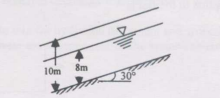
\includegraphics[width=0.3\columnwidth]{figs/q46.png}
\caption*{}
\label{fig:Q.46}
\end{figure}
\begin{enumerate}
\item 0.70
\item 0.80
\item 1.00
\item 1.20
\end{enumerate}

\item Match the following groups.

\hfill{\brak{\text{GATE CE 2007}}}
\begin{table}[H]
\centering
\begin{tabular}{c|c}
Group-I & Group-II \\
\hline
Constant head permeability test & Pile foundations \\
\hline
Consolidation test & Specific gravity \\
\hline
Pycnometer test & Clay soil \\
\hline
Negative skin friction & Sand \\
\end{tabular}
\caption*{}
\label{tab:Q.47}
\end{table}
\begin{enumerate}
\item P-4, Q-3, R-2, S-1
\item P-4, Q-2, R-3, S-1
\item P-3, Q-4, R-2, S-1
\item P-4, Q-1, R-2, S-3
\end{enumerate}

\item The bearing capacity of a rectangular footing of plan dimensions 1.5 m $\times$ 3 m resting on the surface of a sand deposit was estimated as 600 kN/m$^2$ when the water table is far below the base of the footing. The bearing capacities in kN/m$^2$ when the water level rises to depths of 3 m, 1.5 m and 0.5 m below the base of the footing are

\hfill{\brak{\text{GATE CE 2007}}}
\begin{enumerate}
\item 600, 600, 400
\item 600, 450, 350
\item 600, 500, 250
\item 600, 400, 250
\end{enumerate}

\item What is the ultimate capacity in kN of the pile group shown in the figure assuming the group to fail as a single block?

\hfill{\brak{\text{GATE CE 2007}}}
\begin{figure}[H]
\centering
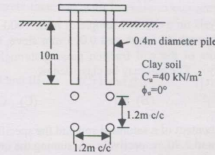
\includegraphics[width=0.3\columnwidth]{figs/q49.png}
\caption*{}
\label{fig:Q.49}
\end{figure}
\begin{enumerate}
\item 921.6
\item 1177.6
\item 2438.6
\item 3481.6
\end{enumerate}

\item A horizontal water jet with a velocity of $10 m/s$ and cross sectional area of $10 mm^2$ strikes a flat plate held normal to the flow direction. The density of water is $1000 kg/m^3$. The total force on the plate due to the jet is

\hfill{\brak{\text{GATE CE 2007}}}
\begin{enumerate}
\item 100 N
\item 10 N
\item 1 N
\item 0.1 N
\end{enumerate}

\item A 1:50 scale model of a spillway is to be tested in the laboratory. The discharge in the prototype is $1000 m^3$/s. The discharge to be maintained in the model test is

\hfill{\brak{\text{GATE CE 2007}}}
\begin{enumerate}
\item $0.057 m^3/s$
\item $0.08 m^3/s$
\item $0.57 m^3/s$
\item $5.7 m^3/s$
\end{enumerate}

\item A triangular open channel has a vertex angle of $90^\circ$ and carries flow at a critical depth of $0.30$ m. The discharge in the channel is

\hfill{\brak{\text{GATE CE 2007}}}
\begin{enumerate}
\item $0.08 m^3/s$
\item $0.11 m^3/s$
\item $0.15 m^3/s$
\item $0.2 m^3/s$
\end{enumerate}

\item Flow rate of a fluid $\brak{text{density}= 1000 kg/m^3}$ in a small diameter tube is $800 mm^3/s$. The length and the diameter of the tube are 2 m and 0.5 mm, respectively. The pressure drop in 2 m length is equal to 2.0 MPa. The viscosity of the fluid is

\hfill{\brak{\text{GATE CE 2007}}}
\begin{enumerate}
\item $0.025 N.s/m^2$
\item $0.012 N.s/m^2$
\item $0.00192 N.s/m^2$
\item $0.00102 N.s/m^2$
\end{enumerate}

\item The flow rate in a wide rectangular open channel is $2.0 m^3/s$ per metre width. The channel bed slope is $0.002$. The Manning’s roughness coefficient is $0.012$. The slope of the channel is classified as

\hfill{\brak{\text{GATE CE 2007}}}
\begin{enumerate}
\item Critical
\item Horizontal
\item Mild
\item Steep
\end{enumerate}

\item The culturable command area for a distributary channel is $20,000$ hectares. Wheat is grown in the entire area and the intensity of irrigation is $50\%$. The \textit{kor} period for wheat is $30$ days and the \textit{kor} water depth is $120$ mm. The outlet discharge for the distributary should be

\hfill{\brak{\text{GATE CE 2007}}}
\begin{enumerate}
\item 2.85 m$^3$/s
\item 3.21 m$^3$/s
\item 4.63 m$^3$/s
\item 5.23 m$^3$/s
\end{enumerate}

\item An isolated 4-hour storm occurred over a catchment as follows

\begin{table}[H]
\centering
\begin{tabular}{|c|c|c|c|c|}
\hline
Time & $1^{st}$ hour & $2^{nd}$ hour & $3^{rd}$ hour & $4^{th}$ hour \\
\hline
Rainfall $\brak{\text{mm}}$ & 9 & 28 & 12 & 7 \\
\hline
\end{tabular}
\caption*{}
\label{tab:Q.56}
\end{table}
The $\phi$ index for the catchment is $10$ mm/h. The estimated runoff depth from the catchment due to the above storm is

\hfill{\brak{\text{GATE CE 2007}}}
\begin{enumerate}
\item 10 mm
\item 16 mm
\item 20 mm
\item 23 mm
\end{enumerate}

\item Two electrostatic precipitators $\brak{\text{ESPs}}$ are in series. The fractional efficiencies of the upstream and downstream ESPs for size $d_p$ are 80\% and 65\%, respectively. What is the overall efficiency of the system for the same $d_p$?

\hfill{\brak{\text{GATE CE 2007}}}
\begin{enumerate}
\item 100\%
\item 93\%
\item 80\%
\item 65\%
\end{enumerate}

\item 50 g of $\mathrm{CO}_2$ and 25 g of $\mathrm{CH}_4$ are produced from the decomposition of municipal solid waste (MSW) with a formula weight of 120 g. What is the average per capita green house gas production in a city of 1 million people with a MSW production rate of 500 ton/day?

\hfill{\brak{\text{GATE CE 2007}}}
\begin{enumerate}
\item 104 g/day
\item 120 g/day
\item 208 g/day
\item 313 g/day
\end{enumerate}

\item The extra widening required for a two-lane national highway at a horizontal curve of 300 m radius, considering a wheel base of 8 m and a design speed of 100 kmph is

\hfill{\brak{\text{GATE CE 2007}}}
\begin{enumerate}
\item 0.42 m
\item 0.62 m
\item 0.82 m
\item 0.92 m
\end{enumerate}

\item While designing a hill road with a ruling gradient of 6\%, if a sharp horizontal curve of 50 m radius is encountered, the compensated gradient at the curve as per the Indian Roads Congress specifications should be

\hfill{\brak{\text{GATE CE 2007}}}
\begin{enumerate}
\item 4.4\%
\item 4.75\%
\item 5.0\%
\item 5.25\%
\end{enumerate}

\item The design speed on a road is 60 kmph. Assuming the driver reaction time of 2.5 seconds and coefficient of friction of pavement surface as 0.35, the required stopping distance for two-way traffic on a single lane road is

\hfill{\brak{\text{GATE CE 2007}}}
\begin{enumerate}
\item 82.1 m
\item 102.4 m
\item 164.2 m
\item 186.4 m
\end{enumerate}

\item The width of the expansion joint is 20 mm in a cement concrete pavement. The laying temperature is $20^\circ$C and the maximum slab temperature in summer is $60^\circ$C. The coefficient of thermal expansion of concrete is $10 \times 10^{-6}$ mm/mm$^\circ$C and the joint filler compresses up to 50\% of the thickness. The spacing between expansion joints should be

\hfill{\brak{\text{GATE CE 2007}}}
\begin{enumerate}
\item 20 m
\item 25 m
\item 30 m
\item 40 m
\end{enumerate}

\item The following data pertains to the number of commercial vehicles per day for the design of a flexible pavement for a national highway as per IRC:37-1984:

\begin{table}[H]
\centering
\begin{tabular}{|c|c|c|}
\hline
Type of commercial vehicle & Number of vehicles per day considering the number of lanes & Vehicle Damage Factor \\
\hline
Two axle trucks & 2000 & 5\\
\hline
Tandem axle truck & 200 & 6\\
\hline
\end{tabular}
\caption*{}
\label{tab:Q.63}
\end{table}

Assuming a traffic growth factor of 7.5\% per annum for both the types of vehicles, the cumulative number of standard axle load repetitions (in million) for a design life of ten years is

\hfill{\brak{\text{GATE CE 2007}}}
\begin{enumerate}
\item 44.6
\item 57.8
\item 62.4
\item 78.7
\end{enumerate}

\item Match the following tests on aggregate and its properties.
\begin{table}[H]
\centering
\begin{tabular}{c|c}
TEST & PROPERTY \\
\hline
Crushing test & Hardness \\
\hline
Los Angeles Abberation test & Shape \\
\hline
Angularity test & Strenght \\
\end{tabular}
\caption*{}
\label{tab:Q.64}
\end{table}
\hfill{\brak{\text{GATE CE 2007}}}
\begin{enumerate}
\item P-2, Q-1, R-4, S-3
\item P-4, Q-2, R-3, S-1
\item P-3, Q-2, R-1, S-4
\item P-4, Q-1, R-2, S-3
\end{enumerate}

\item The plan of a map was photo copied to a reduced size such that a line originally 100 mm, measures 90 mm. The original scale of the plan was 1:1000. The revised scale is

\hfill{\brak{\text{GATE CE 2007}}}
\begin{enumerate}
\item 1:900
\item 1:1111
\item 1:1121
\item 1:1221
\end{enumerate}

\item The following table gives data of consecutive coordinates in respect of a closed theodolite traverse PQRSP.

\begin{table}[H]
\centering
\begin{tabular}{|c|c|c|c|c|}
\hline
Station & Northing, m & Southing, m & Easting, m & Westing, m \\
\hline
P & 400.75 &        &         & 300.5 \\
Q & 100.25 &        & 199.25  &        \\
R &        & 199.0  & 399.75  &        \\
S &        & 300.0  &         & 200.5 \\
\hline
\end{tabular}
\end{table}

The magnitude and direction of error of closure in whole circle bearing are

\hfill{\brak{\text{GATE CE 2007}}}
\begin{enumerate}
\item 2.0 m and $45^\circ$
\item 2.0 m and $315^\circ$
\item 2.82 m and $315^\circ$
\item 3.42 m and $45^\circ$
\end{enumerate}

\item The following measurements were made during testing a levelling instrument.

\begin{table}[H]
\centering
\begin{tabular}{| c | c c |}
\hline
\multirow{2}{*}{Instrument at} & \multicolumn{2}{c|}{Staff Reading at} \\
\cline{2-3}
& $P_1$\hspace{10pt} & $Q_1$\hspace{10pt} \\
\hline
P & 2.800 m & 1.700 m \\
Q & 2.700 m & 1.800 m \\
\hline
\end{tabular}
\end{table}

$P_1$ is close to P and $Q_1$ is close to Q. If the reduced level of station P is 100.000 m, the reduced level of station Q is

\hfill{\brak{\text{GATE CE 2007}}}
\begin{enumerate}
\item 99.000 m
\item 100.000 m
\item 101.000 m
\item 102.000 m
\end{enumerate}

\item Two straight lines intersect at an angle of $60^\circ$. The radius of a curve joining the two straight lines is 600 m. The length of long chord and mid-ordinates in metres of the curve are

\hfill{\brak{\text{GATE CE 2007}}}
\begin{enumerate}
\item 80.4, 600.0
\item 600.0, 80.4
\item 600.0, 39.89
\item 49.89, 300.0
\end{enumerate}

\item The magnetic bearing of a line AB is S $45^\circ$ E and the declination is $5^\circ$ West. The true bearing of the line AB is

\hfill{\brak{\text{GATE CE 2007}}}
\begin{enumerate}
\item S $45^\circ$ E
\item S $40^\circ$ E
\item S $50^\circ$ E
\item S $50^\circ$ W
\end{enumerate}

\section*{COMMON DATA QUESTIONS}

\subsection*{Common Data for Questions 70 and 71:}
Water is flowing through the permeability apparatus as shown in the figure. The coefficient of permeability of the soil is $k m/s$ and the porosity ofthe soil sample is 0.50.

\begin{figure}[H]
\centering
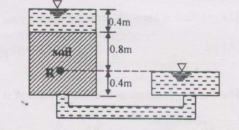
\includegraphics[width=0.5\columnwidth]{figs/q70,71.png}
\caption*{}
\label{fig:Q.70,71}
\end{figure}

\item The total head, elevation head and pressure head in metres of water at the point R shown in the figure are

\hfill{\brak{\text{GATE CE 2007}}}
\begin{enumerate}
\item 0.8, 0.4, 0.4
\item 1.2, 0.4, 0.4
\item 0.4, 0, 0.4
\item 1.6, 0.4, 1.2
\end{enumerate}

\item What are the discharge velocity and seepage velocity through the soil sample?

\hfill{\brak{\text{GATE CE 2007}}}
\begin{enumerate}
\item $k,2k$
\item $\frac{2}{3}k,\frac{4}{3}k$
\item $2k,k$
\item $\frac{4}{3}k,\frac{2}{3}k$
\end{enumerate}

\subsection*{Common Data for Questions 72 and73:}
Ordinates of a 1-hour unit hydrograph at 1 hour intervals, starting from time $t=0$ are 0, 2, 6, 4, 2, 1 and 0 m$^3$/s.

\item Catchment area represented by this unit hydrograph is

\hfill{\brak{\text{GATE CE 2007}}}
\begin{enumerate}
\item $1.0 km^2$
\item $2.0 km^2$
\item $3.2 km^2$
\item $5.4 km^2$
\end{enumerate}

\item Ordinate of a 3-hour unit hydrograph for the catchment at $t=3$ hours is

\hfill{\brak{\text{GATE CE 2007}}}
\begin{enumerate}
\item $2.0 m^3/s$
\item $3.0 m^3/s$
\item $4.0 m^3/s$
\item $5.0 m^3/s$
\end{enumerate}

\subsection*{Common Data for Questions 74 and 75:}
A completely mixed activated sludge process is used to treat a wastewater flow of 1 million litres per day (1 MLD) having a BOD$_5$ of 200 mg/L. The biomass concentration in the aeration tank is 2000 mg/L and the concentration of the net biomass leaving the system is 50 mg/L. The aeration tank has a volume of 200 m$^3$.

\item What is the hydraulic retention time of the wastewater in aeration tank?

\hfill{\brak{\text{GATE CE 2007}}}
\begin{enumerate}
\item 0.2 h
\item 4.8 h
\item 10 h
\item 24 h
\end{enumerate}

\item What is the average time for which the biomass stays in the system?

\hfill{\brak{\text{GATE CE 2007}}}
\begin{enumerate}
\item 5 h
\item 8 h
\item 2 days
\item 8 days
\end{enumerate}

\section*{LINKED ANSWER QUESTIONS: Q.76 to Q.85 carry two marks each.}

\subsection*{Statement for Linked Answer Questions 76 and 77:}
A distributed two span load continuous beam having equal spans each of length L is subjected to a uniformly w per unit length. The beam has constant flexural rigidity.

\item The reaction at the middle support is

\hfill{\brak{\text{GATE CE 2007}}}
\begin{enumerate}
\item $wL$
\item $\dfrac{5wL}{2}$
\item $\dfrac{5wL}{4}$
\item $\dfrac{5wL}{8}$
\end{enumerate}

\item The bending moment of the middle support is

\hfill{\brak{\text{GATE CE 2007}}}
\begin{enumerate}
\item $\dfrac{wL^2}{4}$
\item $\dfrac{wL^2}{8}$
\item $\dfrac{wL^2}{12}$
\item $\dfrac{wL^2}{16}$
\end{enumerate}

\subsection*{Statement for Linked Answer Questions 78 and 79:}
A singly reinforced rectangular concrete beam has a width of 150 mm and an effective depth of 330 mm. The characteristic compressive strength of concrete is $20MPa$ and the characteristic tensile strength of steel is $415MPa$. Adopt the stress block for concrete as given in IS 456-2000 and take limiting value of depth of neutral axis as 0.48 times the effective depth of the beam.

\item The limiting value of the moment of resistance of the beam in kN.m is

\hfill{\brak{\text{GATE CE 2007}}}
\begin{enumerate}
\item 0.14
\item 0.45
\item 45.08
\item 156.82
\end{enumerate}

\item The limiting area of tension steel in $mm^2$ is

\hfill{\brak{\text{GATE CE 2007}}}
\begin{enumerate}
\item 473.9
\item 412.3
\item 373.9
\item 312.3
\end{enumerate}

\subsection*{Statement for Linked Answer Questions 80 and 81:}
The ground conditions at a site are as shown in the figure. The water table at the site which was initially at a depth of 5~m below the ground level got permanently lowered to a depth of 15~m below the ground level due to pumping of water over a few years. Assume the following data:

\begin{enumerate}
\item unit weight of water $= 10$~kN/m$^3$
\item unit weight of sand above water table $= 18$~kN/m$^3$
\item unit weight of sand and clay below the water table $= 20$~kN/m$^3$
\item coefficient of volume compressibility $= 0.25$~m$^2$/MN
\end{enumerate}

\begin{figure}[H]
\centering
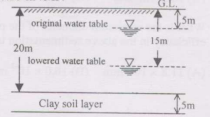
\includegraphics[width=0.5\columnwidth]{figs/q80,81.png}
\caption*{}
\label{fig:Q.81,82}
\end{figure}

\item What is the change in the effective stress in kN/m$^2$ at mid-depth of the clay layer due to the lowering of the water table?

\hfill{\brak{\text{GATE CE 2007}}}
\begin{enumerate}
\item 0
\item 20
\item 80
\item 100
\end{enumerate}

\item What is the compression of the clay layer in mm due to the lowering of the water table?

\hfill{\brak{\text{GATE CE 2007}}}
\begin{enumerate}
\item 125
\item 100
\item 25
\item 0
\end{enumerate}

\subsection*{Statement for Linked Answer Questions 83 and 84:}
A rectangular open channel needs to be designed to carry a flow of $2.0$~m$^3$/s under uniform flow conditions. The Manning’s roughness coefficient is $0.018$. The channel should be such that the flow depth is equal to half the width, and the Froude number is equal to $0.5$.

\item The bed slope of the channel to be provided is

\hfill{\brak{\text{GATE CE 2007}}}
\begin{enumerate}
\item 0.0012
\item 0.0021
\item 0.0025
\item 0.0052
\end{enumerate}

\item Keeping the width, flow depth and roughness the same, if the bed slope of the above channel is doubled, the average boundary shear stress under uniform flow conditions is

\hfill{\brak{\text{GATE CE 2007}}}
\begin{enumerate}
\item $5.6~N/m^2$
\item $10.8~N/m^2$
\item $12.3~N/m^2$
\item $17.2~N/m^2$
\end{enumerate}

\subsection*{Statement for Linked Answer Questions 84 and 85:}
A plain sedimentation tank with a length of 20~m, width of 10~m, and a depth of 3~m is used in a water treatment plant to treat 4 million litres of water per day (4~MLD). The average temperature of water is 20$^\circ$C. The dynamic viscosity of water is $1.002 \times 10^{-3}$~N$\cdot$s/m$^2$ at 20$^\circ$C. Density of water is 998.2~kg/m$^3$. Average specific gravity of particles is 2.65.

\item What is the surface overflow rate in the sedimentation tank?

\hfill{\brak{\text{GATE CE 2007}}}
\begin{enumerate}
\item $20~m^3/m^2/day$
\item $40~m^3/m^2/day$
\item $67~m^3/m^2/day$
\item $133~m^3/m^2/day$
\end{enumerate}

\item What is the minimum diameter of the particle which can be removed with 100\% efficiency in the above sedimentation tank?

\hfill{\brak{\text{GATE CE 2007}}}
\begin{enumerate}
\item 11.8~$\times$~10$^{-3}$~mm
\item 16.0~$\times$~10$^{-3}$~mm
\item 50~$\times$~10$^{-3}$~mm
\item 160~$\times$~10$^{-3}$~mm
\end{enumerate}
\end{enumerate}

\section*{END OF THE QUESTION PAPER}

\end{document}